% =============================================================================
% Phase I — Validation méthodologique sur LunarLander
% =============================================================================
% Inclus via \input{} dans le fichier principal sous \section{Phase I...}
% Hiérarchie interne : \subsection / \subsubsection / \paragraph
% =============================================================================

Avant d'aborder des environnements plus complexes, cette phase préliminaire
vise à maîtriser les outils et pratiques du RL moderne : optimisation
systématique des hyperparamètres, monitoring de la convergence et élagage
automatique des configurations non prometteuses. L'environnement
\textit{LunarLander} de la suite OpenAI Gymnasium constitue un terrain
d'entraînement standard et bien documenté pour valider ces pratiques.

% -----------------------------------------------------------------------------
\subsection{Environnement et algorithmes sélectionnés}
% -----------------------------------------------------------------------------

LunarLander \parencite{GymnasiumDocumentationLunarLander} est un problème de
contrôle classique dans lequel un agent doit poser un module lunaire entre deux
drapeaux situés en (0,0) en gérant sa poussée et son orientation. Deux
variantes sont disponibles :

\begin{itemize}
  \item \textbf{LunarLander (discret)} : l'agent choisit à chaque pas de
        temps parmi quatre actions discrètes (ne rien faire, allumer le
        propulseur gauche, principal ou droit).
  \item \textbf{LunarLanderContinuous (continu)} : l'espace d'action est
        continu et bidimensionnel, correspondant à l'intensité de chaque
        propulseur.
\end{itemize}

\begin{figure}[h!]
  \centering
  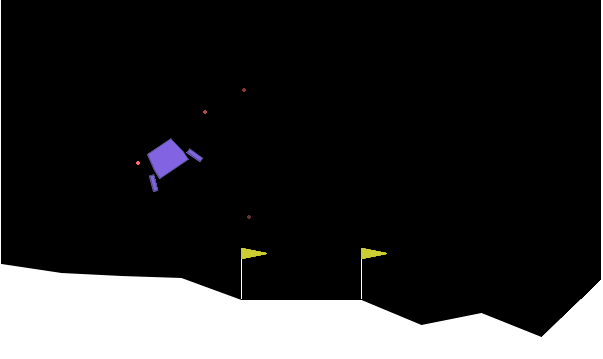
\includegraphics[width=0.8\textwidth]{img/lunar_lander.png}
  \caption{Aperçu de l'environnement LunarLander}
  \label{fig:lunar_lander}
\end{figure}

L'espace d'observation est identique dans les deux cas : un vecteur de huit
variables continues décrivant la position, la vitesse, l'angle, la vitesse
angulaire et le contact des deux pattes avec le sol.

La fonction de récompense pénalise la consommation de carburant et la distance
à la zone d'atterrissage, et accorde un bonus lors du contact des pattes avec
le sol ainsi qu'une récompense de $+100$ pour un atterrissage réussi (ou une
pénalité de $-100$ pour un crash). L'épisode se termine soit à
l'atterrissage, soit au crash, soit lors d'une sortie du terrain de jeu. Un
épisode est considéré \textbf{résolu} lorsque la récompense atteint
$\geq 200$.

Ce choix se justifie par plusieurs raisons : LunarLander est suffisamment
complexe pour nécessiter un réglage soigneux des hyperparamètres, disponible
en variantes discrète et continue (permettant de comparer des algorithmes de
natures différentes), et constitue un benchmark de référence largement utilisé
dans la littérature, facilitant la mise en perspective des résultats.

Trois algorithmes ont été sélectionnés pour couvrir les principales familles
du RL profond :

\begin{itemize}
  \item \textbf{DQN} (\textit{Deep Q-Network})
        \parencite{mnihHumanlevelControlDeep2015} : algorithme
        \textit{off-policy} basé sur la Q-valeur, applicable uniquement aux
        espaces d'action discrets. Évalué sur la variante
        \textit{LunarLander}.

  \item \textbf{PPO} (\textit{Proximal Policy Optimization})
        \parencite{schulmanProximalPolicyOptimization2017} : algorithme
        \textit{on-policy} de type acteur-critique, applicable aux deux types
        d'espaces d'action. Évalué sur les deux variantes.

  \item \textbf{SAC} (\textit{Soft Actor-Critic})
        \parencite{haarnojaSoftActorCriticOffPolicy2018} : algorithme
        \textit{off-policy} à entropie maximale, conçu pour les espaces
        d'action continus. Évalué sur la variante
        \textit{LunarLanderContinuous}.
\end{itemize}

Ce choix permet de comparer un algorithme à valeur (DQN), un algorithme
\textit{on-policy} (PPO) et un algorithme \textit{off-policy} à entropie
maximale (SAC), qui représentent trois approches fondamentalement différentes
du problème d'apprentissage par renforcement.

% -----------------------------------------------------------------------------
\subsection{Optimisation des hyperparamètres}
% -----------------------------------------------------------------------------

\subsubsection{Cadre général}

L'optimisation des hyperparamètres est réalisée avec le framework
\textbf{Optuna} \parencite{akibaOptunaNextgenerationHyperparameter2019}, en
utilisant le sampler \textit{Tree-structured Parzen Estimator} (TPE). TPE est
un algorithme bayésien qui modélise séparément la distribution des bons et des
mauvais hyperparamètres, et dirige la recherche vers les régions prometteuses
de l'espace de configuration. Chaque configuration est évaluée sur
\textbf{250\,000 pas de temps} d'entraînement, suivie d'une évaluation
déterministe sur \textbf{20 épisodes}. La métrique optimisée est la récompense
moyenne obtenue lors de cette évaluation finale.

\subsubsection{Élagage des essais non concluants}

Afin de réduire le coût computationnel, un \textbf{MedianPruner} est
appliqué : il interrompt prématurément tout essai dont la performance
intermédiaire (évaluée toutes les 10\,000 steps) est inférieure à la médiane
des essais précédents au même stade d'entraînement. Deux paramètres encadrent
ce mécanisme :

\begin{itemize}
  \item \texttt{n\_startup\_trials = 15} : les 15 premiers essais sont
        toujours complétés afin de fournir suffisamment de données au pruner
        pour établir une médiane de référence fiable avant d'activer l'élagage.
  \item \texttt{n\_warmup\_steps = 30\,000} : au sein d'un essai, l'élagage
        ne peut s'activer qu'après 30\,000 steps, laissant le temps à
        l'agent d'amorcer sa convergence avant d'être jugé.
\end{itemize}

Un essai interrompu par le pruner est enregistré avec l'état \texttt{PRUNED}
dans la base Optuna et comptabilisé dans le total des essais effectués, au
même titre qu'un essai complet. Seuls les essais ayant échoué pour des raisons
techniques (crash, erreur mémoire) ne sont pas comptabilisés. La campagne
cible au minimum \textbf{150 essais} par combinaison algorithme/environnement.

\subsubsection{Hyperparamètres testés}
\label{sec:hparams}

Les tableaux suivants décrivent les hyperparamètres testés pour chaque
algorithme, leur rôle et les plages de recherche utilisées. Pour l'ensemble
des expériences, la politique neuronale repose sur des perceptrons
multicouches (\texttt{MlpPolicy} dans Stable-Baselines3). L'espace
d'observation de LunarLander étant un vecteur de huit dimensions, l'usage de
réseaux convolutifs n'est pas pertinent dans ce contexte.

% Colonnes : col 1 fixée, col 3 fixée, col 2 prend le reste exact de \textwidth.
% 6\tabcolsep = 2 séparateurs × 3 colonnes. Garantit l'absence de débordement.
\newlength{\hpColA}\setlength{\hpColA}{3.6cm}
\newlength{\hpColC}\setlength{\hpColC}{3.0cm}

% ── DQN ───────────────────────────────────────────────────────────────────────
\begingroup
\footnotesize
\setlength{\tabcolsep}{8pt}
\renewcommand{\arraystretch}{1.4}
\begin{longtable}{%
  p{\hpColA}%
  p{\dimexpr\textwidth - \hpColA - \hpColC - 6\tabcolsep\relax}%
  p{\hpColC}%
}
  \caption{Hyperparamètres testés pour DQN}
  \label{tab:hparams_dqn}\\
  \toprule
  \textbf{Hyperparamètre} & \textbf{Rôle} & \textbf{Plage / valeurs}\\
  \midrule
\endfirsthead
  \multicolumn{3}{l}{\footnotesize\itshape Suite du tableau \ref{tab:hparams_dqn}}\\[2pt]
  \toprule
  \textbf{Hyperparamètre} & \textbf{Rôle} & \textbf{Plage / valeurs}\\
  \midrule
\endhead
  \midrule
  \multicolumn{3}{r}{\footnotesize\itshape Suite page suivante}\\
\endfoot
  \bottomrule
\endlastfoot

\texttt{learning\_rate}
  & Pas de gradient de l'optimiseur Adam (\textit{continu, log}).
    Une valeur trop élevée déstabilise l'entraînement~; trop faible,
    la convergence est lente.
  & $[10^{-5},\;10^{-3}]$ \\[4pt]
\texttt{buffer\_size}
  & Taille du \textit{replay buffer} (\textit{catégoriel}).
    Un buffer plus grand améliore la diversité des transitions
    échantillonnées, au coût d'une empreinte mémoire plus importante.
  & $\{10^4,\;5{\cdot}10^4,\;10^5\}$ \\[4pt]
\texttt{learning\_starts}
  & Nombre de pas avant le début des mises à jour (\textit{catégoriel}).
    Permet de pré-remplir le buffer avec des transitions aléatoires
    pour stabiliser les premières itérations.
  & $\{0,\;1000,\;5000\}$ \\[4pt]
\texttt{batch\_size}
  & Nombre de transitions échantillonnées à chaque mise à jour
    (\textit{catégoriel}).
  & $\{32,\;64,\;128,\;256\}$ \\[4pt]
\texttt{gamma}
  & Facteur d'actualisation des récompenses futures (\textit{catégoriel}).
    Proche de 1~: l'agent est prévoyant~; proche de 0~: il privilégie
    les récompenses immédiates.
  & $\{0.90,\ldots,0.999\}$ \\[4pt]
\texttt{train\_freq}
  & Fréquence des mises à jour en nombre de pas de temps
    (\textit{catégoriel}).
  & $\{1,\;4,\;8,\;16\}$ \\[4pt]
\texttt{target\_update\_interval}
  & Nombre de mises à jour entre deux synchronisations du réseau cible
    (\textit{catégoriel}). Le \textit{target network} stabilise
    l'apprentissage en fixant temporairement les valeurs cibles.
  & $\{100,\;250,\;500,\;1000\}$ \\[4pt]
\texttt{exploration\_fraction}
  & Fraction du training durant laquelle $\varepsilon$ décroît de sa
    valeur initiale à sa valeur finale (\textit{continu}).
  & $[0.05,\;0.5]$ \\[4pt]
\texttt{exploration\_final\_eps}
  & Valeur minimale de $\varepsilon$ après la phase d'exploration
    (\textit{continu}). Correspond au taux d'actions aléatoires résiduel
    en exploitation.
  & $[0.01,\;0.1]$ \\[4pt]
\texttt{net\_arch}
  & Architecture du réseau MLP --- nombre et taille des couches
    cachées (\textit{catégoriel}).
  & \textit{small} [64,64],\newline
    \textit{medium} [256,256],\newline
    \textit{large} [400,300] \\
\end{longtable}
\endgroup

% ── PPO ───────────────────────────────────────────────────────────────────────
\begingroup
\footnotesize
\setlength{\tabcolsep}{8pt}
\renewcommand{\arraystretch}{1.4}
\begin{longtable}{%
  p{\hpColA}%
  p{\dimexpr\textwidth - \hpColA - \hpColC - 6\tabcolsep\relax}%
  p{\hpColC}%
}
  \caption{Hyperparamètres testés pour PPO}
  \label{tab:hparams_ppo}\\
  \toprule
  \textbf{Hyperparamètre} & \textbf{Rôle} & \textbf{Plage / valeurs}\\
  \midrule
\endfirsthead
  \multicolumn{3}{l}{\footnotesize\itshape Suite du tableau \ref{tab:hparams_ppo}}\\[2pt]
  \toprule
  \textbf{Hyperparamètre} & \textbf{Rôle} & \textbf{Plage / valeurs}\\
  \midrule
\endhead
  \midrule
  \multicolumn{3}{r}{\footnotesize\itshape Suite page suivante}\\
\endfoot
  \bottomrule
\endlastfoot

\texttt{learning\_rate}
  & Pas de gradient de l'optimiseur Adam (\textit{continu, log}).
  & $[10^{-5},\;10^{-3}]$ \\[4pt]
\texttt{n\_steps}
  & Nombre de pas collectés avant chaque mise à jour de la politique,
    \textit{rollout length} (\textit{catégoriel}). Doit être supérieur
    à \texttt{batch\_size}~--- les configurations invalides sont rejetées
    automatiquement lors du sampling.
  & $\{256,\;512,\;1024,\;2048\}$ \\[4pt]
\texttt{batch\_size}
  & Taille des mini-batchs utilisés pour les mises à jour
    (\textit{catégoriel}).
  & $\{32,\;64,\;128,\;256,\;512\}$ \\[4pt]
\texttt{n\_epochs}
  & Nombre de passes sur les données collectées à chaque mise à jour
    (\textit{catégoriel}). Augmenter ce nombre améliore l'utilisation des
    données mais peut déstabiliser la politique.
  & $\{1,\;3,\;5,\;10,\;20\}$ \\[4pt]
\texttt{gamma}
  & Facteur d'actualisation des récompenses futures (\textit{catégoriel}).
  & $\{0.90,\ldots,0.999\}$ \\[4pt]
\texttt{gae\_lambda}
  & Paramètre $\lambda$ du \textit{Generalized Advantage Estimation} (GAE)
    (\textit{catégoriel}). Contrôle le compromis biais-variance dans
    l'estimation de l'avantage.
  & $\{0.80,\ldots,1.0\}$ \\[4pt]
\texttt{ent\_coef}
  & Coefficient de la prime d'entropie (\textit{continu, log}).
    Encourage l'exploration en pénalisant les politiques trop
    déterministes.
  & $[10^{-8},\;0.1]$ \\[4pt]
\texttt{clip\_range}
  & Paramètre $\varepsilon$ de la contrainte PPO (\textit{catégoriel}).
    Limite l'écart entre l'ancienne et la nouvelle politique lors des
    mises à jour.
  & $\{0.1,\;0.2,\;0.3,\;0.4\}$ \\[4pt]
\texttt{max\_grad\_norm}
  & Norme maximale du gradient --- \textit{gradient clipping}
    (\textit{continu, log}). Prévient les mises à jour explosives et
    stabilise l'entraînement.
  & $[0.3,\;5.0]$ \\[4pt]
\texttt{vf\_coef}
  & Coefficient de la perte du critique (\textit{continu}). Contrôle
    l'importance relative de l'erreur de prédiction de valeur par rapport
    à la perte de politique.
  & $[0.1,\;1.0]$ \\[4pt]
\texttt{net\_arch}
  & Architecture du réseau MLP acteur-critique (\textit{catégoriel}).
  & \textit{small} [64,64],\newline
    \textit{medium} [256,256],\newline
    \textit{large} [400,300] \\
\end{longtable}
\endgroup

% ── SAC ───────────────────────────────────────────────────────────────────────
\begingroup
\footnotesize
\setlength{\tabcolsep}{8pt}
\renewcommand{\arraystretch}{1.4}
\begin{longtable}{%
  p{\hpColA}%
  p{\dimexpr\textwidth - \hpColA - \hpColC - 6\tabcolsep\relax}%
  p{\hpColC}%
}
  \caption{Hyperparamètres testés pour SAC}
  \label{tab:hparams_sac}\\
  \toprule
  \textbf{Hyperparamètre} & \textbf{Rôle} & \textbf{Plage / valeurs}\\
  \midrule
\endfirsthead
  \multicolumn{3}{l}{\footnotesize\itshape Suite du tableau \ref{tab:hparams_sac}}\\[2pt]
  \toprule
  \textbf{Hyperparamètre} & \textbf{Rôle} & \textbf{Plage / valeurs}\\
  \midrule
\endhead
  \midrule
  \multicolumn{3}{r}{\footnotesize\itshape Suite page suivante}\\
\endfoot
  \bottomrule
\endlastfoot

\texttt{learning\_rate}
  & Pas de gradient commun aux réseaux acteur et critique
    (\textit{continu, log}).
  & $[10^{-5},\;10^{-3}]$ \\[4pt]
\texttt{buffer\_size}
  & Taille du \textit{replay buffer} (\textit{catégoriel}).
  & $\{10^4,\;5{\cdot}10^4,\;10^5\}$ \\[4pt]
\texttt{learning\_starts}
  & Nombre de pas avant le début des mises à jour (\textit{catégoriel}).
  & $\{1000,\;5000,\;10000\}$ \\[4pt]
\texttt{batch\_size}
  & Taille des mini-batchs pour les mises à jour (\textit{catégoriel}).
  & $\{32,\;64,\;128,\;256,\;512\}$ \\[4pt]
\texttt{gamma}
  & Facteur d'actualisation des récompenses futures (\textit{catégoriel}).
  & $\{0.90,\ldots,0.999\}$ \\[4pt]
\texttt{tau}
  & Taux de mise à jour \textit{soft} du réseau cible (\textit{catégoriel}).
    À chaque pas~:
    $\theta_{\text{cible}} \leftarrow \tau\,\theta + (1-\tau)\,\theta_{\text{cible}}$.
  & $\{0.001,\;0.005,\;0.01,\;0.02,\;0.05\}$ \\[4pt]
\texttt{ent\_coef}
  & Coefficient d'entropie géré automatiquement (\texttt{auto}) : SAC
    ajuste ce coefficient à chaque pas de gradient pour maintenir une
    entropie cible $\mathcal{H}^* = -\dim(\mathcal{A})$, définie par
    \cite{haarnojaSoftActorCriticAlgorithms2019} comme l'opposé de la
    dimension de l'espace d'action.
  & \texttt{auto} \\[4pt]
\texttt{use\_sde}
  & Active l'\textit{State Dependent Exploration} (SDE)
    (\textit{catégoriel}). Le bruit d'exploration dépend de l'état courant
    ce qui peut améliorer l'exploration dans les
    espaces d'action continus. Ce bruit est maintenu pendant plusieurs steps consécutifs. Des trajectoires entières peuvent ainsi être explorées.
  & $\{\text{True},\;\text{False}\}$ \\[4pt]
\texttt{target\_update\_interval}
  & Nombre de gradient steps entre deux mises à jour du réseau cible
    (\textit{catégoriel}).
  & $\{1,\;2,\;4\}$ \\[4pt]
\texttt{net\_arch}
  & Architecture des réseaux MLP acteur et critique (\textit{catégoriel}).
  & \textit{small} [64,64],\newline
    \textit{medium} [256,256],\newline
    \textit{large} [400,300] \\
\end{longtable}
\endgroup

% -----------------------------------------------------------------------------
\subsection{Résultats de l'optimisation}
% -----------------------------------------------------------------------------

Cette section présente les résultats obtenus pour chaque algorithme sur les
deux variantes de l'environnement LunarLander, en mettant en lumière les
configurations optimales identifiées et leur robustesse à travers les
différentes seeds.
 
% ── Synthèse des scores Optuna ────────────────────────────────────────────────
 
Le tableau~\ref{tab:scores_optuna} présente les scores obtenus par la
meilleure configuration de chaque combinaison algorithme/environnement à
l'issue de la phase de tuning. Ces scores correspondent à la récompense
moyenne sur 20 épisodes déterministes, obtenue par le meilleur essai parmi
les 150 évalués sur 250\,000 steps. Ils constituent un indicateur du
potentiel maximal de chaque configuration, indépendamment de sa robustesse
inter-seeds --- qui fait l'objet de la section~\ref{sec:eval_finale}.
 
\begin{table}[h!]
\centering
\footnotesize
\renewcommand{\arraystretch}{1.3}
\caption{Score Optuna des meilleures configurations (récompense moyenne sur
         20 épisodes déterministes, meilleur essai parmi 150)}
\label{tab:scores_optuna}
\begin{tabular}{llr}
  \toprule
  \textbf{Algorithme} & \textbf{Variante} & \textbf{Score Optuna} \\
  \midrule
  DQN & Discret  & $275.14$ \\
  PPO & Discret  & $278.76$ \\
  PPO & Continu  & $280.42$ \\
  SAC & Continu  & $284.05$ \\
  \bottomrule
\end{tabular}
\end{table}
 
Les quatre configurations dépassent largement le seuil de résolution officiel
de 200, ce qui confirme l'efficacité du protocole d'optimisation. SAC obtient
le meilleur score sur la variante continue, tandis que les deux variantes PPO
se situent dans un écart inférieur à 2 points, suggérant une robustesse de
l'algorithme aux deux types d'espaces d'action sur cet environnement.
 
% Colonnes des tableaux d'hyperparamètres optimaux :
%   col 1 fixée à \hpOptA, col 2 prend le reste exact de \textwidth.
%   4\tabcolsep = 2 séparateurs × 2 colonnes.
\newlength{\hpOptA}\setlength{\hpOptA}{5.5cm}
 
% -----------------------------------------------------------------------------
\subsubsection{DQN --- LunarLander discret}
% -----------------------------------------------------------------------------
 
\begingroup
\footnotesize
\setlength{\tabcolsep}{8pt}
\renewcommand{\arraystretch}{1.4}
\begin{longtable}{%
  p{\hpOptA}%
  p{\dimexpr\textwidth - \hpOptA - 4\tabcolsep\relax}%
}
  \caption{Hyperparamètres optimaux --- DQN / discret (score Optuna : 275.14)}
  \label{tab:hparams_opt_dqn}\\
  \toprule
  \textbf{Hyperparamètre} & \textbf{Valeur optimale} \\
  \midrule
\endfirsthead
  \multicolumn{2}{l}{\footnotesize\itshape Suite du tableau \ref{tab:hparams_opt_dqn}}\\[2pt]
  \toprule
  \textbf{Hyperparamètre} & \textbf{Valeur optimale} \\
  \midrule
\endhead
  \bottomrule
\endlastfoot
 
\texttt{learning\_rate}           & $4.73 \times 10^{-4}$ \\
\texttt{buffer\_size}             & $10^{4}$ \\
\texttt{learning\_starts}         & $5\,000$ \\
\texttt{batch\_size}              & $64$ \\
\texttt{gamma}                    & $0.99$ \\
\texttt{train\_freq}              & $1$ \\
\texttt{target\_update\_interval} & $250$ \\
\texttt{exploration\_fraction}    & $0.253$ \\
\texttt{exploration\_final\_eps}  & $0.075$ \\
\texttt{net\_arch}                & \textit{medium} $[256,\;256]$ \\
\end{longtable}
\endgroup
 
\medskip
 
La configuration optimale retenue pour DQN présente deux caractéristiques
notables. D'une part, la taille du \textit{replay buffer} ($10^4$) est
inférieure aux valeurs typiques de la littérature ($10^5$ à $10^6$
\parencite{mnihHumanlevelControlDeep2015}). Cette valeur s'explique
vraisemblablement par le budget limité de la phase de tuning (250\,000 steps)
: avec un petit buffer, les transitions récentes dominent l'échantillonnage,
ce qui peut accélérer la convergence à court terme mais reste à confirmer sur
les 500\,000 steps de l'évaluation finale. D'autre part, \texttt{train\_freq
= 1} implique une mise à jour du réseau à chaque pas de temps, ce qui, combiné
au petit buffer, produit un ratio mise-à-jour/données élevé. Cette
configuration agressive a convergé efficacement sur cet environnement, mais
introduit potentiellement une variance plus importante dans les gradients.
 
% -----------------------------------------------------------------------------
\subsubsection{PPO --- LunarLander discret}
% -----------------------------------------------------------------------------
 
\begingroup
\footnotesize
\setlength{\tabcolsep}{8pt}
\renewcommand{\arraystretch}{1.4}
\begin{longtable}{%
  p{\hpOptA}%
  p{\dimexpr\textwidth - \hpOptA - 4\tabcolsep\relax}%
}
  \caption{Hyperparamètres optimaux --- PPO / discret (score Optuna : 278.76)}
  \label{tab:hparams_opt_ppo_disc}\\
  \toprule
  \textbf{Hyperparamètre} & \textbf{Valeur optimale} \\
  \midrule
\endfirsthead
  \multicolumn{2}{l}{\footnotesize\itshape Suite du tableau \ref{tab:hparams_opt_ppo_disc}}\\[2pt]
  \toprule
  \textbf{Hyperparamètre} & \textbf{Valeur optimale} \\
  \midrule
\endhead
  \bottomrule
\endlastfoot
 
\texttt{learning\_rate} & $2.37 \times 10^{-4}$ \\
\texttt{n\_steps}       & $2\,048$ \\
\texttt{batch\_size}    & $256$ \\
\texttt{n\_epochs}      & $20$ \\
\texttt{gamma}          & $0.995$ \\
\texttt{gae\_lambda}    & $0.98$ \\
\texttt{ent\_coef}      & $1.55 \times 10^{-2}$ \\
\texttt{clip\_range}    & $0.4$ \\
\texttt{max\_grad\_norm}& $2.13$ \\
\texttt{vf\_coef}       & $0.889$ \\
\texttt{net\_arch}      & \textit{large} $[400,\;300]$ \\
\end{longtable}
\endgroup
 
\medskip
 
La configuration PPO discrète se distingue par un \texttt{clip\_range} de
$0.4$, valeur maximale de la plage explorée et nettement supérieure à la
valeur standard de $0.2$ \parencite{schulmanProximalPolicyOptimization2017}.
Un \texttt{clip\_range} élevé autorise des mises à jour de politique plus
importantes à chaque gradient step, tout en conservant la garantie de
stabilité propre à PPO grâce au mécanisme de clipping. Cette valeur, associée
à \texttt{n\_epochs = 20} et \texttt{n\_steps = 2048}, indique que PPO effectue $\lfloor 2048 / 256 \rfloor = 8$ mini-batches\footnote{256 étant la taille d'un batch} par époque, soit 160 mises à jour du réseau pour chaque rollout de 2048 transitions.
 
% -----------------------------------------------------------------------------
\subsubsection{PPO --- LunarLanderContinuous}
% -----------------------------------------------------------------------------
 
\begingroup
\footnotesize
\setlength{\tabcolsep}{8pt}
\renewcommand{\arraystretch}{1.4}
\begin{longtable}{%
  p{\hpOptA}%
  p{\dimexpr\textwidth - \hpOptA - 4\tabcolsep\relax}%
}
  \caption{Hyperparamètres optimaux --- PPO / continu (score Optuna : 280.42)}
  \label{tab:hparams_opt_ppo_cont}\\
  \toprule
  \textbf{Hyperparamètre} & \textbf{Valeur optimale} \\
  \midrule
\endfirsthead
  \multicolumn{2}{l}{\footnotesize\itshape Suite du tableau \ref{tab:hparams_opt_ppo_cont}}\\[2pt]
  \toprule
  \textbf{Hyperparamètre} & \textbf{Valeur optimale} \\
  \midrule
\endhead
  \bottomrule
\endlastfoot
 
\texttt{learning\_rate} & $6.42 \times 10^{-5}$ \\
\texttt{n\_steps}       & $2\,048$ \\
\texttt{batch\_size}    & $32$ \\
\texttt{n\_epochs}      & $10$ \\
\texttt{gamma}          & $0.995$ \\
\texttt{gae\_lambda}    & $0.98$ \\
\texttt{ent\_coef}      & $1.27 \times 10^{-4}$ \\
\texttt{clip\_range}    & $0.4$ \\
\texttt{max\_grad\_norm}& $1.65$ \\
\texttt{vf\_coef}       & $0.105$ \\
\texttt{net\_arch}      & \textit{large} $[400,\;300]$ \\
\end{longtable}
\endgroup
 
\medskip
 
La comparaison entre les deux variantes PPO révèle une convergence vers des
valeurs communes pour plusieurs hyperparamètres structurels
(\texttt{n\_steps = 2048}, \texttt{gae\_lambda = 0.98},
\texttt{clip\_range = 0.4}, \texttt{net\_arch = large}), ce qui suggère que
ces choix sont robustes à la nature de l'espace d'action sur cet
environnement. En revanche, deux hyperparamètres diffèrent significativement
entre les deux variantes : le \texttt{learning\_rate} est quatre fois plus
faible pour la variante continue ($6.42 \times 10^{-5}$ contre
$2.37 \times 10^{-4}$), et l'\texttt{ent\_coef} est deux ordres de grandeur
inférieur ($1.27 \times 10^{-4}$ contre $1.55 \times 10^{-2}$). Ces
différences indiquent que l'optimisation d'une politique gaussienne en espace
continu requiert des mises à jour plus prudentes et une pression d'exploration
entropique moindre que dans le cas discret.
 
% -----------------------------------------------------------------------------
\subsubsection{SAC --- LunarLanderContinuous}
% -----------------------------------------------------------------------------
 
\begingroup
\footnotesize
\setlength{\tabcolsep}{8pt}
\renewcommand{\arraystretch}{1.4}
\begin{longtable}{%
  p{\hpOptA}%
  p{\dimexpr\textwidth - \hpOptA - 4\tabcolsep\relax}%
}
  \caption{Hyperparamètres optimaux --- SAC / continu (score Optuna : 284.05)}
  \label{tab:hparams_opt_sac}\\
  \toprule
  \textbf{Hyperparamètre} & \textbf{Valeur optimale} \\
  \midrule
\endfirsthead
  \multicolumn{2}{l}{\footnotesize\itshape Suite du tableau \ref{tab:hparams_opt_sac}}\\[2pt]
  \toprule
  \textbf{Hyperparamètre} & \textbf{Valeur optimale} \\
  \midrule
\endhead
  \bottomrule
\endlastfoot
 
\texttt{learning\_rate}           & $9.95 \times 10^{-4}$ \\
\texttt{buffer\_size}             & $10^{5}$ \\
\texttt{learning\_starts}         & $1\,000$ \\
\texttt{batch\_size}              & $512$ \\
\texttt{gamma}                    & $0.99$ \\
\texttt{tau}                      & $0.05$ \\
\texttt{ent\_coef}                & \texttt{auto} \\
\texttt{use\_sde}                 & \texttt{True} \\
\texttt{target\_update\_interval} & $2$ \\
\texttt{net\_arch}                & \textit{medium} $[256,\;256]$ \\
\end{longtable}
\endgroup
 
\medskip
 
SAC obtient le meilleur score Optuna ($284.05$) avec une architecture de
réseau \textit{medium} $[256, 256]$, plus petite que celle retenue par PPO
(\textit{large} $[400, 300]$), ce qui illustre l'efficacité par paramètre
propre aux algorithmes \textit{off-policy} bénéficiant du \textit{replay
buffer}. Deux hyperparamètres méritent d'être soulignés. D'une part,
\texttt{tau = 0.05} est la valeur maximale de la plage testée, dix fois
supérieure à la valeur standard de $0.005$
\parencite{haarnojaSoftActorCriticOffPolicy2018} : cette mise à jour rapide
du réseau cible favorise une convergence accélérée sur un environnement de
faible dimensionnalité comme LunarLander, où le risque de divergence lié à
un réseau cible instable est limité. D'autre part, \texttt{use\_sde = True}
confirme l'intérêt de l'\textit{State Dependent Exploration} pour les espaces
d'action continus : le bruit d'exploration structuré en fonction de l'état
permet une exploration plus cohérente que le bruit gaussien indépendant de l'état.

% -----------------------------------------------------------------------------
\subsection{Évaluation finale multi-seeds}
\label{sec:eval_finale}
% -----------------------------------------------------------------------------

% -----------------------------------------------------------------------------
\subsubsection{Protocole d'évaluation finale}
% -----------------------------------------------------------------------------

Une fois les hyperparamètres optimaux identifiés pour chaque combinaison
algorithme/environnement, une évaluation finale est conduite pour mesurer la
robustesse des configurations retenues. Chaque modèle est réentraîné
\textbf{from scratch} sur \textbf{5 seeds indépendantes}
($\{42,\ 123,\ 456,\ 789,\ 1337\}$) avec 500\,000 pas de temps
d'entraînement, puis évalué sur 20 épisodes.

\paragraph{Évaluation déterministe.}
L'évaluation est conduite en mode \textbf{déterministe}, ce qui diffère du
comportement adopté durant l'entraînement selon l'algorithme :

\begin{itemize}
  \item \textbf{PPO} : pendant l'entraînement, PPO échantillonne ses actions
        depuis une distribution de probabilités (gaussienne pour le continu,
        catégorielle pour le discret) afin d'explorer. En mode déterministe,
        l'action retenue est le \textit{mode} de cette distribution ---
        l'action de probabilité maximale --- sans aucun échantillonnage.

  \item \textbf{SAC} : de même, SAC paramétrise une distribution gaussienne
        et échantillonne lors de l'entraînement pour maximiser l'entropie.
        En mode déterministe, il retourne la moyenne de cette distribution,
        ce qui correspond à la politique la plus probable sans bruit
        d'exploration.

  \item \textbf{DQN} : le mode déterministe consiste à sélectionner
        systématiquement l'action de Q-valeur maximale (argmax), avec
        $\varepsilon = 0$. C'est déjà le comportement naturel de DQN
        lors de l'exploitation ; le mode déterministe ne change donc pas
        fondamentalement la politique évaluée.
\end{itemize}

Ce choix d'évaluation déterministe est standard dans la littérature RL : il
mesure la politique \textit{apprise} sans bruit d'exploration, offrant une
estimation plus fidèle des performances en déploiement réel.

\paragraph{Métriques rapportées.}
Les métriques suivantes sont calculées sur les 20 épisodes d'évaluation, puis
agrégées sur les 5 seeds :

\begin{itemize}
  \item Récompense moyenne et écart-type inter-seeds,
  \item Récompense minimale et maximale observées,
  \item Taux de succès : fraction d'épisodes avec une récompense $\geq 200$
        (seuil de résolution officiel de LunarLander),
  \item Nombre de seeds pour lesquelles la récompense moyenne atteint le seuil
        de résolution.
\end{itemize}

Cette procédure multi-seeds permet de distinguer les configurations robustes
--- qui convergent systématiquement --- des configurations qui réussissent de
manière occasionnelle en raison de la stochasticité de l'entraînement.

% -----------------------------------------------------------------------------
\subsubsection{Résultats de l'évaluation multi-seeds}
\label{sec:eval_finale}
% -----------------------------------------------------------------------------

Les résultats de l'évaluation multi-seeds sont présentés dans le
tableau~\ref{tab:eval_finale}. Chaque configuration optimale est réentraînée
sur 5 seeds indépendantes ($\{42, 123, 456, 789, 1337\}$) pendant 500\,000
steps, puis évaluée de manière déterministe sur 20 épisodes. Les métriques
rapportées sont la récompense moyenne et son écart-type inter-seeds (std
échantillon, $n-1$), les récompenses extrêmes observées, le taux de succès
(fraction d'épisodes avec une récompense $\geq 200$) et le nombre de seeds
pour lesquelles la récompense moyenne dépasse le seuil de résolution.

\begin{table}[h!]
\centering
\footnotesize
\setlength{\tabcolsep}{5pt}
\renewcommand{\arraystretch}{1.3}
\caption{Résultats de l'évaluation multi-seeds (500\,000 steps,
         récompense moyenne sur 20 épisodes déterministes, std échantillon)}
\label{tab:eval_finale}
\newlength{\evalColB}\setlength{\evalColB}{3.2cm}
\newlength{\evalColSide}\setlength{\evalColSide}{1.4cm}
\begin{tabular}{%
  p{1.5cm}%
  p{1.5cm}%
  p{\evalColB}%
  p{\evalColSide}%
  p{\evalColSide}%
  p{\evalColSide}%
  p{\evalColSide}%
}
\toprule
\textbf{Algo.} & \textbf{Env.}
  & \textbf{Mean $\pm$ Std}
  & \textbf{Min}
  & \textbf{Max}
  & \textbf{Succès}
  & \textbf{Seeds} \\
\midrule
DQN & Discret  & $145.19 \pm 45.76$ & $101.26$ & $231.89$ & $39\%$ & $1/5$ \\
PPO & Discret  & $218.58 \pm 50.72$ & $143.95$ & $278.76$ & $77\%$ & $3/5$ \\
PPO & Continu  & $208.67 \pm 50.17$ & $159.60$ & $278.96$ & $74\%$ & $2/5$ \\
SAC & Continu  & $233.44 \pm 52.50$ & $132.67$ & $281.01$ & $79\%$ & $4/5$ \\
\bottomrule
\end{tabular}
\end{table}

\paragraph{SAC et PPO --- configurations robustes.}
SAC obtient la meilleure récompense moyenne ($233.44 \pm 52.50$) et le taux
de succès le plus élevé ($79\%$, 4 seeds sur 5 résolues), confirmant la
supériorité de l'algorithme à entropie maximale sur la variante continue.
PPO affiche des performances solides dans les deux variantes, avec des
récompenses moyennes supérieures au seuil de résolution ($218.58$ en discret,
$208.67$ en continu) et des taux de succès proches de $75\%$. La variante
discrète résout légèrement plus de seeds (3/5 contre 2/5), bien que les scores
moyens soient proches, ce qui suggère une variance inter-seeds plus favorable
en espace discret.

\paragraph{DQN --- fragilité de la configuration optimale.}
DQN présente un écart marqué entre son score Optuna ($275.14$) et sa
récompense moyenne en évaluation finale ($145.19$), soit une chute de plus de
130 points. Cet écart s'explique vraisemblablement par la nature de la
configuration retenue : un \textit{replay buffer} de $10^4$ transitions et
un \texttt{train\_freq = 1} constituent une configuration agressive, optimisée
pour converger rapidement sur 250\,000 steps de tuning, mais qui ne se
généralise pas sur les 500\,000 steps de l'évaluation finale. Le ratio élevé
mise-à-jour/données induit une variance importante dans les gradients, ce qui
se traduit par une instabilité inter-seeds (écart-type de $45.76$, une seule
seed résolue sur 5).

\paragraph{Écarts-types élevés --- limite de l'évaluation à 5 seeds.}
Les écarts-types inter-seeds sont importants pour tous les algorithmes
($45$--$52$ points), ce qui reflète la stochasticité inhérente à
l'entraînement par renforcement. Avec seulement 5 seeds, ces estimations
restent bruitées. Cette phase ayant pour vocation la validation du protocole
d'optimisation plutôt qu'une évaluation exhaustive, ce nombre de seeds est
néanmoins suffisant pour dégager les tendances principales.

\begin{figure}[h!]
\centering
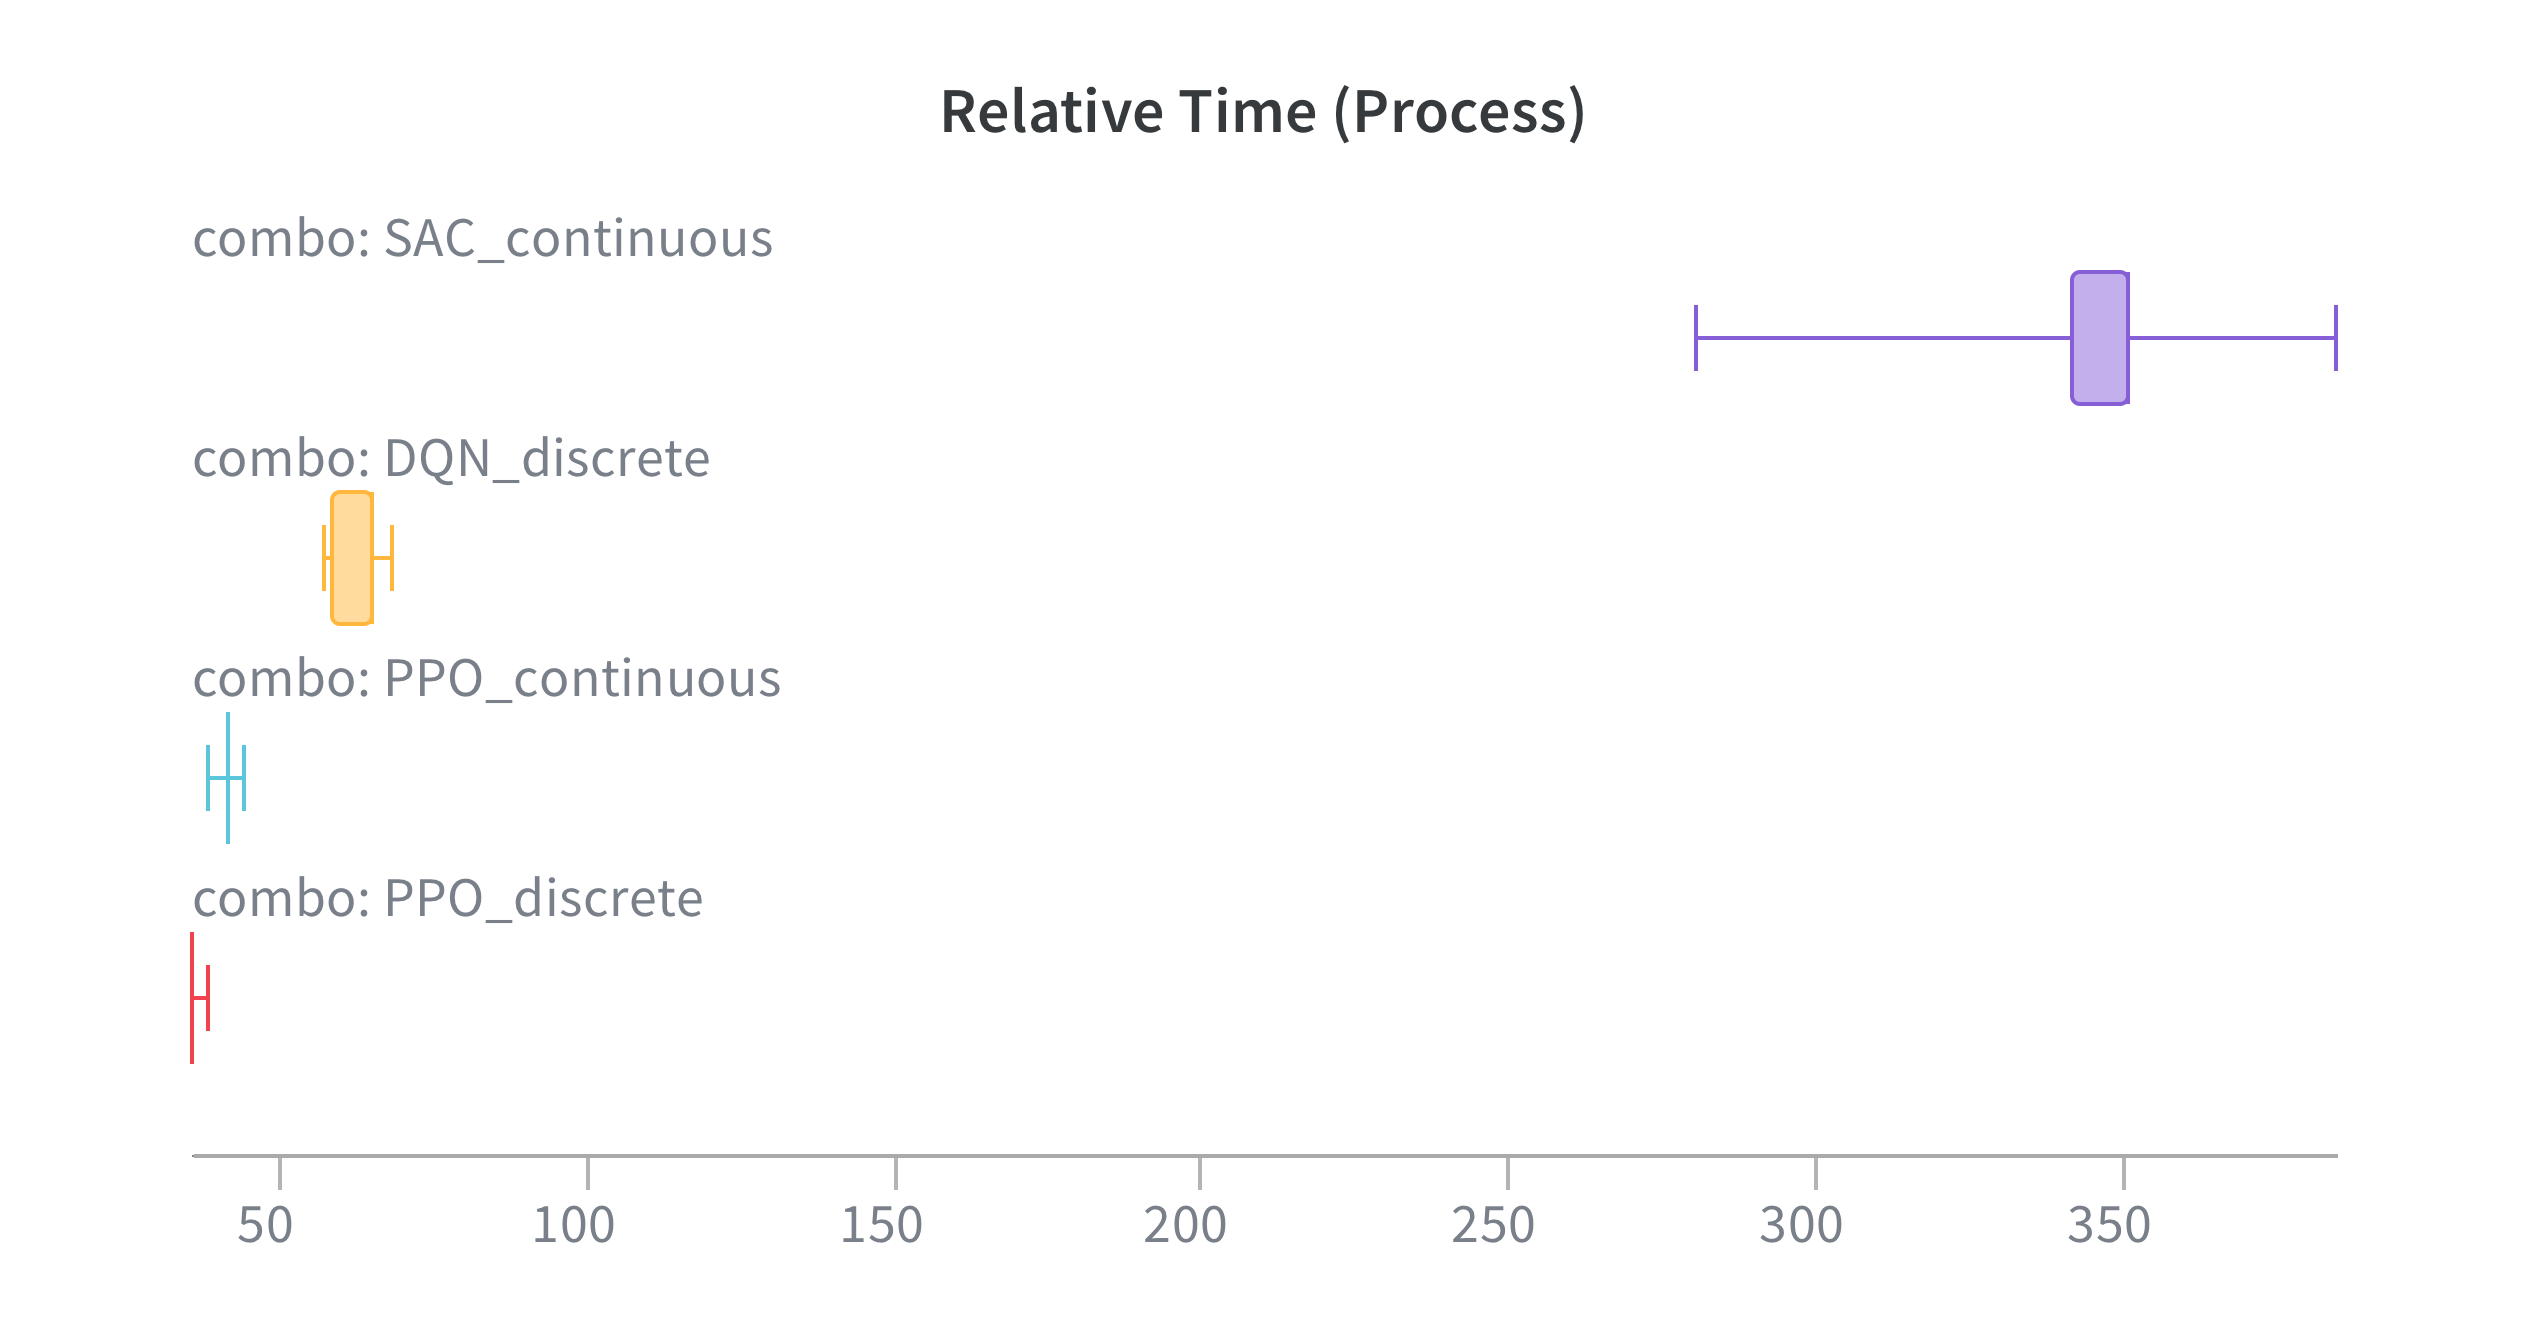
\includegraphics[width=\textwidth]{img/model_convergence_boxplot.png}
\caption{Distribution du temps de convergence (en minutes) pour chaque
         combinaison algorithme/environnement, sur les 5 seeds indépendantes.}
\label{fig:convergence_boxplot}
\end{figure}

La figure~\ref{fig:convergence_boxplot} illustre la distribution des temps
de convergence inter-seeds. SAC requiert globalement un temps d'entraînement
plus important que PPO et DQN, ce qui s'explique par le coût computationnel
de ses mises à jour : SAC maintient simultanément deux réseaux Q (double
critic) et un acteur, et calcule à chaque step la mise à jour du coefficient
d'entropie adaptatif --- un coût par update structurellement plus élevé que
celui des autres algorithmes, indépendamment de la fréquence des mises à jour.
Il est important de mettre en évidence que ces tests ont été réalisés sur un cluster avec des ressources partagées et donc les modèles n'ont pas forcément été entraînés dans des conditions strictement identiques, ce qui peut introduire une variance supplémentaire dans les temps de convergence observés. Cependant, la tendance générale reste claire : SAC est plus coûteux en temps d'entraînement que PPO et DQN, ce qui doit être pris en compte dans le choix de l'algorithme en fonction des contraintes de ressources disponibles.

\paragraph{Synthèse.}
Ces résultats mettent en évidence deux enseignements principaux. D'une part,
le score Optuna n'est pas un prédicteur fiable de la robustesse inter-seeds :
DQN en est l'illustration la plus nette, avec le deuxième meilleur score de
tuning mais les performances finales les plus faibles. D'autre part, SAC et
PPO représentent des compromis distincts : SAC offre les meilleures
performances sur la variante continue au prix d'un coût computationnel plus
élevé, tandis que PPO, applicable aux deux types d'espaces d'action avec des
performances stables, constitue un choix plus polyvalent pour des contextes
aux ressources limitées.